%%% NEW STUFF %%%

\begin{frame}[fragile,label=SubgroupLattice]{Subgroup Lattice Basics}
Let $U$ and $H$ be subgroups of a finite group.
  \begin{itemize}
  \item<1-> By $UH$ we mean the \emph{set} $\{ u h \mid u\in U, h\in H\}$.\\[6pt]
  \item<2-> $U \join V = \<U,H\>$ means the group generated by $U$ and $H$.\\[6pt]
  \item<3-> $UH \subseteq \<U,H\>$ and 
    equality holds iff $U$ and $H$ permute: 
    \[
    UH = \<U,H\> \quad \Leftrightarrow \quad U H = H U.
    \]
  \end{itemize}
\visible<4->{
\begin{center}
  \begin{tikzpicture}[scale=.4]
    \node (H) at (4,4) [fill,circle,inner sep=\dotsize] {}; \draw (H) node [right] {$H$};
    \node (U) at (-4,4) [fill,circle,inner sep=\dotsize] {}; \draw (U) node [left] {$U$};
    \node (U0) at (0,0) [fill,circle,inner sep=\dotsize] {}; 
    \draw (1.5,-.75) node {$U_0 = U\cap H$};
    \node (UH) at (0,8) [fill,circle,inner sep=\dotsize] {}; \draw (UH) node [above] {$\<U,H\>$};
 \draw
    (U) to [out=-10,in=100] (U0) to [out=170,in=-80] (U)
    (UH) to [out=-10,in=100] (H) to [out=170,in=-80] (UH)
    (H) to [out=190,in=80] (U0) to [out=10,in=-100] (H)
    (UH) to [out=190,in=80] (U) to [out=10,in=-100] (UH);
    \visible<5->{\shade[top color=olivegreen,bottom color=gray!50] 
      (U) to [out=-10,in=100] (U0) to [out=170,in=-80] (U);
      \draw (-7,0) node {$[U_0,U]:=\{V \mid U_0 \leq V \leq U\}$};}
    \visible<6->{  \shade[top color=blue,bottom color=gray!50] 
      (UH) to [out=-10,in=100] (H) to [out=170,in=-80] (UH);
      \draw (7,6) node {$[H, \<U,H\>]$};}
    \visible<5->{ \node (V) at (-1.6,1.8) [fill,circle,inner sep=\dotsize] {};
      \draw (-2,2) node {$V$};}
    \end{tikzpicture}
\end{center}
}
\end{frame}

\begin{frame}[fragile,label=SubgroupLattice,shrink=5]{Interval Isomorphisms}
  \begin{columns}
    \begin{column}{0.3\textwidth}
      \begin{center}
        \begin{tikzpicture}[scale=.3]
              \node (H) at (4,4) [draw,circle,inner sep=\dotsize] {}; \draw (H) node [right] {$H$};
    \node (U) at (-4,4) [draw,circle,inner sep=\dotsize] {}; \draw (U) node [left] {$U$};
    \node (U0) at (0,0) [draw,circle,inner sep=\dotsize] {}; 
    \draw (1.5,-.75) node {$U_0 = U\cap H$};
    \node (UH) at (0,8) [draw,circle,inner sep=\dotsize] {}; \draw (UH) node
    [above] {$UH$};
 \draw
    (U) to [out=-10,in=100] (U0) to [out=170,in=-80] (U)
    (UH) to [out=-10,in=100] (H) to [out=170,in=-80] (UH)
    (H) to [out=190,in=80] (U0) to [out=10,in=-100] (H)
    (UH) to [out=190,in=80] (U) to [out=10,in=-100] (UH);

    \visible<2>{\shade[top color=olivegreen,bottom color=gray!-45] 
      (U) to [out=-10,in=100] (U0) to [out=170,in=-80] (U);}
    \visible<5->{
      \fill[color=olivegreen] 
      (U) to [out=-10,in=100] (U0) to [out=170,in=-80] (U);}
    \visible<2,5->{  \shade[top color=olivegreen,bottom color=gray!-45] 
      (UH) to [out=-10,in=100] (H) to [out=170,in=-80] (UH);}
    \visible<6->{\fill[color=orange]    
      (H) to [out=190,in=80] (U0) to [out=10,in=-100] (H);}
    \visible<6->{\shade[top color=orange,bottom color=gray!0]    
      (UH) to [out=190,in=80] (U) to [out=10,in=-100] (UH);}
       \end{tikzpicture}
      \end{center}
    \end{column}
    \begin{column}{0.7\textwidth}
      \begin{itemize}
      \item<1-> Assume $H\subnormal \<U, H\>$.
        \uncover<2->{
          \[
          \text{Then } \; UH = \<U, H\> \; \text{ and  } \; [U_0, U] \cong [H, UH].
          \]}
        \item<3-> Now drop assumption $H\subnormal \<U,H\>$,\\[4pt]
          assume $UH = \<U,H\>$, and define   
          \begin{equation*}
            %      \label{eq:dedekind-1}
            [U_0, U]^H := \{ V\in [U_0,U] \mid VH = HV\}.
          \end{equation*}
          the \alert{$H$-permuting subgroups}.
          \vskip2mm 
        \item<4-> If $U \subnormal UH$,
          define
          \begin{equation*}
            %  \label{eq:dedekind-2}
            [U_0, U]_H := \{ V\in [U_0,U] \mid H\leq N_{UH}(V)\}, 
          \end{equation*}
          the \alert{$H$-invariant subgroups}: 
          $h \, V \,h^{-1} = V$ for all $h\in H$.
      \end{itemize}
    \end{column}
  \end{columns}
\vskip-2mm

  \visible<5->{
%The main result relating these sets to $[H, UH]$ is
    % Lemma on H-invariant isomorphic intervals
    \begin{lemma}
      \label{lemma-wjd-4}
      \begin{enumerate}
      \item $[H, UH]  \cong  [U_0, U]^H \leq [U_0, U]$ \only<6>{ and \hskip2mm $[U, UH]
        \cong  [U_0, H]^U \leq [U_0, H]$}
\\[6pt]
      \item If $U \subnormal UH$, then  $[U_0, U]_H  = [U_0, U]^H \leq [U_0, U]$.\\[6pt]
      \item If $H \subnormal UH$,  then  $[U_0, U]_H  = [U_0, U]^H = [U_0, U]$.
      \end{enumerate}
    \end{lemma}
}
\note{
  \begin{itemize}
  \item 
  Since $G=UH$ is a group, the hypothesis of (ii) is equivalent to
$H\leq N_G(U)$, and the hypothesis of (iii) is equivalent to $U\leq N_G(H)$.
\item Part (i) of the lemma says that when two subgroups permute, we can
identify the interval above either one of them with the sublattice of
subgroups below the other that permute with the first.
\item Part (ii) is similar except we identify the interval above $H$ with
the  sublattice of $H$-invariant subgroups below $U$.
\item Once we have proved (i), the
proof of (iii) follows trivially from the Noether isomorphism theorem.
  \end{itemize}}

\end{frame}


\begin{frame}[fragile,label=Dedekind]{Dedekind's Rule}
The proof relies on the following modular law for subgroups:

\vskip3mm

\begin{theorem}[Dedekind's rule]
  \label{lemma-dedekind}
Let $A, B, C$ be subgroups of $G$ with $A\leq B$.  Then,
%% \begin{align*}
%% %\label{eq:dedekind1}
%% A(C\cap B) &= AC \cap B,\qquad \text{ and }\\
%% %\label{eq:dedekind2}
%% (C\cap B)A &= CA \cap B.
%% \end{align*}
\[
A(C\cap B) = AC \cap B \quad \text{ and }
\quad (C\cap B)A = CA \cap B.
\]
\end{theorem}

\vskip3mm

In other words, no pentagons.
\note{Draw picture of $N_5$ with $A\leq B$ to demonstrate that it contradicts Dedekind's rule.}
\end{frame}

\begin{frame}[fragile,label=ProofOfIntervalIsomorphism,shrink=5]{Proof of Interval Isomorphism Lemma}
  \begin{columns}
    \begin{column}{0.4\textwidth}
      {\bf Claim:} $[H, UH]  \cong  [U_0, U]^H \leq [U_0, U]$.

\vskip5mm

      \begin{center}
        \begin{tikzpicture}[scale=.3]
              \node (H) at (4,4) [draw,circle,inner sep=\dotsize] {}; \draw (H) node [right] {$H$};
    \node (U) at (-4,4) [draw,circle,inner sep=\dotsize] {}; \draw (U) node [left] {$U$};
    \node (U0) at (0,0) [draw,circle,inner sep=\dotsize] {}; 
    \draw (1.5,-.75) node {$U_0 = U\cap H$};
    \node (UH) at (0,8) [draw,circle,inner sep=\dotsize] {}; \draw (UH) node
    [above] {$UH$};
 \draw
    (U) to [out=-10,in=100] (U0) to [out=170,in=-80] (U)
    (UH) to [out=-10,in=100] (H) to [out=170,in=-80] (UH)
    (H) to [out=190,in=80] (U0) to [out=10,in=-100] (H)
    (UH) to [out=190,in=80] (U) to [out=10,in=-100] (UH);

          \fill[color=olivegreen] 
          (U) to [out=-10,in=100] (U0) to [out=170,in=-80] (U);
          \shade[top color=olivegreen,bottom color=gray!-45] 
          (UH) to [out=-10,in=100] (H) to [out=170,in=-80] (UH);
          \node (V) at (-2.3,2.5) [fill,circle,inner sep=\dotsize] {};
          \node (VH) at (1.7,6.5){};
          \draw (-2.7,2.9) node {$V$};
          \node (X) at (2.5,5.3) [fill,circle,inner sep=\dotsize] {};
          \node (UcapX) at (-1.5,1.3){};
          \draw (3,5.2) node {$X$};
          \draw[semithick,dotted] 
          (V) to [out=65,in=-155] (VH)
          (X) to [out=-155,in=65] (UcapX);
        \end{tikzpicture}
      \end{center}
    \end{column}
    \begin{column}{0.7\textwidth}
      \begin{itemize}
      \item<1-> 
        The following maps are inverse order isomorphisms:
        \begin{align*}
          \phi: \;& [H, UH] \ni X \mapsto U\cap X \in [U_0, U]^H\\[6pt]
          \psi: \;& [U_0, U]^H \ni V \mapsto VH \in [H, UH].
        \end{align*}
        \begin{itemize}
        \item<2-> Fix $X\in [H, UH]$.  By Dedekind's rule,
          \[
          (U\cap X) H = UH \cap X= HU \cap X = H(U \cap X),
          \]
          so $U\cap X \in [U_0, U]^H$.\\[6pt]
        \item<3->For $V\in [U_0, U]^H$, $VH = HV$ implies $VH \in [H, UH]$. \\[6pt]
        \item<4->  $\psi \circ \phi$ and 
          $\phi \circ \psi$ are the identity maps:
          \[
          \psi \circ \phi (X) = (U\cap X)H =UH \cap X = X,
          \]
          \[
          \phi \circ \psi(V)= VH \cap U =V(H\cap U)= V.
          \]
        \item<5->The maps are order preserving:
          \[X\leq Y \; \Rightarrow \; U\cap X \leq U\cap Y\]
          \[V\leq W \; \Rightarrow \; VH \leq WH.\]
          So, $\phi$ and $\psi$ are inverse order isomorphisms.
        \end{itemize}

      \item<6-> $[U_0, U]^H$ is a sublattice of $[U_0,U]$.

      \end{itemize}
    \end{column}
  \end{columns}
  %\vskip2mm

\end{frame}





\begin{frame}[fragile,label=L7second]{The Exceptional Seven Element Lattice}
  \begin{center}
    {\scalefont{.75}
      \begin{tikzpicture}[scale=.7]
              \node (J1) at (0,1)  [draw, circle, inner sep=\dotsize] {};
      \draw (.36, 1) node {$J_1$};
      \node (H) at (1,0)  [draw, circle, inner sep=\dotsize] {};
      \draw (1.16, -.2) node {$H$};
      \node (M2) at (1,2)  [draw, circle, inner sep=\dotsize] {};
      \draw (1.4, 2) node {$M_2$};
      \node (J2) at (2,1)  [draw, circle, inner sep=\dotsize] {};
      \draw (2.2, .8) node {$J_2$};
      \node (G) at (2,3)  [draw, circle, inner sep=\dotsize] {};
      \draw (2.3, 3.1) node {$G$};
      \node (M1) at (3,2)  [draw, circle, inner sep=\dotsize] {};
      \draw (3.35, 2) node {$M_1$};
      \node (K) at (-1,1.2)  [draw, circle, inner sep=\dotsize] {};
      \draw (-1.28, 1.15) node {$K$};

      \draw[semithick] (H) to (J1) to (M2) to (G) to (M1) to (J2) to (H) (J2) to (M2);
      \draw[semithick] (H) to (K) to (G);

      \end{tikzpicture}
    }
  \end{center}

\begin{theorem}
\label{thm:except-seven-elem}
Suppose $H<G$, $\core_G(H) = 1$, and 
$L_7 \cong [H,G]$.  Then
\begin{enumerate}[(i)]
\item<1-> $G$ is a primitive permutation group.
\item<1-> If $N\ssubnormal G$, then $C_G(N) = 1$.
\item<1-> $G$ contains no non-trivial abelian normal subgroup.
\item<1-> $G$ is not solvable.
\item<1-> $G$ is subdirectly irreducible.
\item<1-> With the possible exception of at most one maximal subgroup, $M_1$ or $M_2$,
  all proper subgroups in the interval $[H,G]$ are core-free. 

%% The three subgroups in $[H,G]$ which cover $H$ (the atoms) are
%%   core-free.  At least one two of the three maximal subgroups (the co-atoms) in
%%   the interval are core-free. 
\end{enumerate}
\end{theorem}
%% \note{  It is obvious that 
%%   \begin{itemize}
%%   \item (ii) $\Rightarrow$ (iii) $\Rightarrow$ (iv), and  
%% \item (ii) $\Rightarrow$ (v), but we include these for
%%   emphasis;
%% \item the hard work is in proving (ii) and (vi), but
%%   the main goal is the pair of restrictions (iii) and (v), which allow us to rule
%%   out a number of the O'Nan-Scott types describing primitive permutation
%%   groups. 
%%   \end{itemize}}
\end{frame}

\begin{frame}[fragile,label=IdeaOfL7Proof]{Idea of the proof}
    %% \begin{column}{0.3\textwidth}
      \begin{center}
        {\scalefont{.78}
          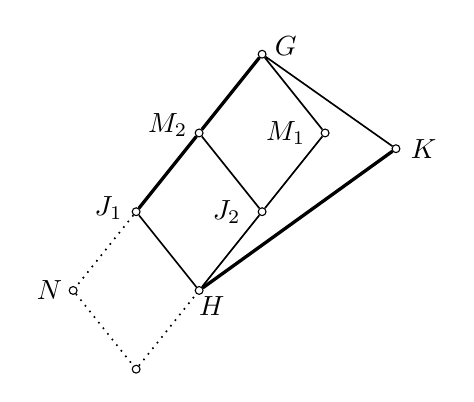
\begin{tikzpicture}[scale=1]
      \node (N) at (-.6,0)  [draw, circle, inner sep=1pt] {};
      \draw (-.9, 0) node {$N$};
      \node (NcapH) at (.2,-1)  [draw, circle, inner sep=1pt] {};
      \node (J1) at (0.2,1)  [draw, circle, inner sep=1pt] {};
      \draw (-.15, 1.05) node {$J_1$};
      \node (H) at (1,0)  [draw, circle, inner sep=1pt] {};
      \draw (1.16, -.2) node {$H$};
      \node (M2) at (1,2)  [draw, circle, inner sep=1pt] {};
      \draw (.6, 2.1) node {$M_2$};
      \node (J2) at (1.8,1)  [draw, circle, inner sep=1pt] {};
      \draw (1.35, 1.) node {$J_2$};
      \node (G) at (1.8,3)  [draw, circle, inner sep=1pt] {};
      \draw (2.1, 3.1) node {$G$};
      \node (M1) at (2.6,2)  [draw, circle, inner sep=1pt] {};
      \draw (2.1, 2) node {$M_1$};
      \node (K) at (3.5,1.8)  [draw, circle, inner sep=1pt] {};
      \draw (3.85, 1.8) node {$K$};
      \draw[semithick,dotted] (J1) to (N) to (NcapH) to (H);
      \visible<4->{\draw[very thick] (J1) to (M2) to (G) (H) to (K);}
      \draw[semithick] (J1) to (M2) to (G) (H) to (K);
      \draw[semithick] (H) to (J1) to (M2) to (G) to (M1) to (J2) to (H) to (K)
      to (G) (J2) to (M2);
    \end{tikzpicture}
 }
\end{center}
      
  %%   \end{column}
  %% \end{columns}

  %% \begin{columns}
  %%   \begin{column}{0.7\textwidth}
      {\bf Claim:} 
      $J_1$ and $J_2$ are core-free subgroups of $G$.\\[6pt]
      {\bf Proof:}
      \begin{itemize}
      \item<2->
      If $N\ssubnormal G$ then $NH$ permutes with each subgroup containing $H$.  
      \note{Let $H \leq X \leq G$.  Then $NHX = NX = XN= XHN = XNH$.}
      \item<3-> If $1\neq N\leq J_1$, then $NH = J_1$, so $J_1$ and $K$ permute.
      \item<4-> Since $J_1K = G$ and $J_1\cap K = H$, our lemma yields
      \[
        [J_1, G] \cong [H, K]^{J_1} = \{X \in[H, K] \mid J_1X=XJ_1 \}.
        \]
   \uncover<5->{Impossible!}
      \end{itemize}

    %% \end{column}


\end{frame}

\begin{frame}[fragile,label=OSTheorem]{Achbacher-O'Nan-Scott Theorem}
Let $G$ be a primitive permutation
group of degree $d$, and let $N := \Soc(G) \cong T^m$ with $m \geq 1$. 
Then one of the following holds.
\vskip2mm
\begin{enumerate}
\item 
$N$ is regular and
  \begin{itemize}
  \item 
  \alert{Affine type} $T$ is cyclic of order $p$, so $|N| = p^m$ . Then 
$d = p^m$ and $G$ is permutation isomorphic to a subgroup of the affine
general linear group $\AGL(m,p)$.
\vskip2mm
\item \alert{Twisted wreath product type} $m \geq 6$, the group $T$ is 
  nonabelian and $G$ is a group of \emph{twisted wreath product type}, with
  $d = |T|^m$.
  \end{itemize}
\vskip2mm
\item $N$ is non-regular, non-abelian, and
  \begin{itemize}
  \item 
\alert{Almost simple} $m = 1$ and $T \leq G \leq \Aut(T)$.
\vskip2mm
\item \alert{Product action} $m \geq 2$ and $G$ is permutation isomorphic to a
subgroup of the product action wreath product $P \wr S_{m/l}$ of degree
$d = nm/l$. The group $P$ is primitive of type 2.(a) or 2.(c), $P$ has
degree $n$ and $\Soc(P) \cong T^l$, where $l \geq 1$ divides $m$.
\vskip2mm
\item 
\alert{Diagonal type} $m \geq 2$ and $T^m \leq G \leq T^m . (\Out(T ) \times S_m)$, with
the diagonal action. The degree $d = |T|^{m-1}$.
  \end{itemize}
\end{enumerate}
\end{frame}

\setbeamercovered{invisible}

\begin{frame}[fragile,label=FinalConclusions]{Conclusions}
  \begin{itemize}
  \item<1-5> We have new methods for building new finite algebras out of
    old so that the congruence lattice changes in predictable ways.
\vskip2mm
  \item<2-5> Using these and other methods we have found representations for all
    finite lattices with at most 7 elements with one exception, thus
    idetifying the unique smallest lattice for which there's no known
    representation. 
\vskip2mm
  \item<3-5> We developed techniques for putting restrictions on groups that
    have certain lattices as intervals in their subgroup lattices.
\vskip2mm
\item<4-5> By studying the lattice $L_7$, we can restrict the class of
  groups which could possibly represent this lattice.  (We believe a slightly
  modified versoin of this lattice will restrict to the class of almost simple
  groups.)
\vskip2mm
\item<5-5> Future work: Restrict to almost simple groups and then solve the problem using the CFSG Theorem.
  \end{itemize}
  %% \vskip5mm 
  %% \visible<4>{
  %%   \hskip-5mm          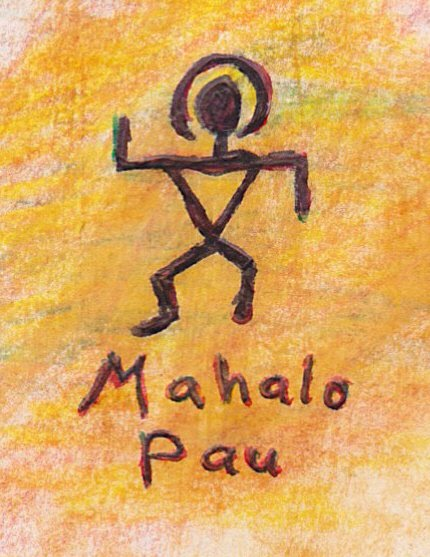
\includegraphics[height=2in]{MahaloPau}
  %% }
\end{frame}
\begin{frame}[fragile,label=FinalConclusions]{}
  \begin{center}
  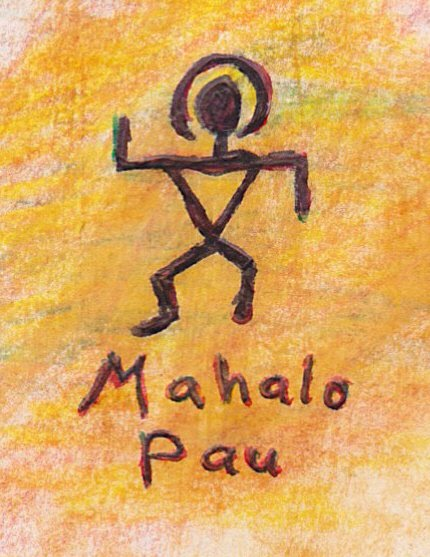
\includegraphics[height=2in]{MahaloPau}
  \end{center}
\end{frame}
